\PassOptionsToPackage{unicode=true}{hyperref} % options for packages loaded elsewhere
\PassOptionsToPackage{hyphens}{url}
%
\documentclass[]{article}
\usepackage{lmodern}
\usepackage{amssymb,amsmath}
\usepackage{ifxetex,ifluatex}
\usepackage{fixltx2e} % provides \textsubscript
\ifnum 0\ifxetex 1\fi\ifluatex 1\fi=0 % if pdftex
  \usepackage[T1]{fontenc}
  \usepackage[utf8]{inputenc}
  \usepackage{textcomp} % provides euro and other symbols
\else % if luatex or xelatex
  \usepackage{unicode-math}
  \defaultfontfeatures{Ligatures=TeX,Scale=MatchLowercase}
\fi
% use upquote if available, for straight quotes in verbatim environments
\IfFileExists{upquote.sty}{\usepackage{upquote}}{}
% use microtype if available
\IfFileExists{microtype.sty}{%
\usepackage[]{microtype}
\UseMicrotypeSet[protrusion]{basicmath} % disable protrusion for tt fonts
}{}
\IfFileExists{parskip.sty}{%
\usepackage{parskip}
}{% else
\setlength{\parindent}{0pt}
\setlength{\parskip}{6pt plus 2pt minus 1pt}
}
\usepackage{hyperref}
\hypersetup{
            pdftitle={Numerical investigation of two-phase flow in high-permeability porous media Effect of permeability variation on traction terms},
            pdfauthor={Maxime Cochennec¹; Hossein Davarzani¹* (h.davarzani@brgm.fr); Yohan Davit²; Ioannis Ignatiadis¹; Michel Quintard²},
            pdfborder={0 0 0},
            breaklinks=true}
\urlstyle{same}  % don't use monospace font for urls
\usepackage{longtable,booktabs}
% Fix footnotes in tables (requires footnote package)
\IfFileExists{footnote.sty}{\usepackage{footnote}\makesavenoteenv{longtable}}{}
\usepackage{graphicx,grffile}
\makeatletter
\def\maxwidth{\ifdim\Gin@nat@width>\linewidth\linewidth\else\Gin@nat@width\fi}
\def\maxheight{\ifdim\Gin@nat@height>\textheight\textheight\else\Gin@nat@height\fi}
\makeatother
% Scale images if necessary, so that they will not overflow the page
% margins by default, and it is still possible to overwrite the defaults
% using explicit options in \includegraphics[width, height, ...]{}
\setkeys{Gin}{width=\maxwidth,height=\maxheight,keepaspectratio}
\setlength{\emergencystretch}{3em}  % prevent overfull lines
\providecommand{\tightlist}{%
  \setlength{\itemsep}{0pt}\setlength{\parskip}{0pt}}
\setcounter{secnumdepth}{0}
% Redefines (sub)paragraphs to behave more like sections
\ifx\paragraph\undefined\else
\let\oldparagraph\paragraph
\renewcommand{\paragraph}[1]{\oldparagraph{#1}\mbox{}}
\fi
\ifx\subparagraph\undefined\else
\let\oldsubparagraph\subparagraph
\renewcommand{\subparagraph}[1]{\oldsubparagraph{#1}\mbox{}}
\fi

% set default figure placement to htbp
\makeatletter
\def\fps@figure{htbp}
\makeatother

\usepackage{setspace}
\usepackage{cleveref}
\usepackage{xcolor}
\doublespacing

\title{Numerical investigation of two-phase flow in high-permeability porous
media Effect of permeability variation on traction terms}
\author{Maxime Cochennec¹ \and Hossein Davarzani¹* (h.davarzani@brgm.fr) \and Yohan Davit² \and Ioannis Ignatiadis¹ \and Michel Quintard²}
\date{\today{}}

\begin{document}
\maketitle

¹French Geological Survey, Orléans, France ²Institut de Mécanique des
Fluides de Toulouse, Toulouse, France

*To whom correspondence should be addressed

\begin{center}\rule{0.5\linewidth}{\linethickness}\end{center}

\hypertarget{abstract}{%
\section{Abstract}\label{abstract}}

In this paper we study the effects of varying permeability on traction
terms exerted at the different boundaries for two-phase flow in
Hele-Shaw cell. The traction terms, or surface force, are. surface
integrals that are necessary to close the continuous macroscopic
momentum balance equations for two-phase flow in porous media. These
terms are usually modeled from experimental results or obtained by
solving a closure problem (a set of boundary value problems to solve on
a representative periodic unit-cell). Here these terms are calculated
directly by means of direct numerical simulations, and the value of
these terms on each interface is studied as a function of the varying
permeability and capillary number. We focus on two-phase displacement in
high-permeability porous media for which the characteristic flow regimes
implies a non-negligible extent of the fluid-fluid interface and thus;

\hypertarget{introduction}{%
\section{Introduction}\label{introduction}}

\hypertarget{two-phase-flow-in-high-permeability-porous-media}{%
\subsection{Two-phase flow in high-permeability porous
media}\label{two-phase-flow-in-high-permeability-porous-media}}

An accurate description of two-phase flow in high-permeability porous
media is of major importance for several practical applications. One can
mention, among others, soil remediation in gravely soils
{[}\protect\hyperlink{ref-fetter2017contaminant}{1}{]}, nuclear safety
{[}\protect\hyperlink{ref-clavier2017modeling}{2}{]} or hydrodynamic of
catalytic fixed bed reactors
{[}\protect\hyperlink{ref-Santos1991}{3}{]}. However, most of the
literature is dedicated to two-phase flow in low-permeability porous
media.

Due to the larger pore size, two-phase flow in high-permeability porous
media (hereafter, high-permeability porous media refers to media for
which the characteristic particle diameter is about one millimeter and
above) results in a complex interaction between capillary, gravity and
viscous forces {[}\protect\hyperlink{ref-davit2018one}{4}{]}. Because of
this complex interplay, the characteristic flow regimes are very
different from those observed for surface tension dominated flow
{[}\protect\hyperlink{ref-dullien2012porous}{5}{]}. For low-permeability
medium, if the surface tension between the fluids is not too low and the
viscosity not too high, that is the capillary number is low (usually
inferior to \(10^{-3}\)), the fluid repartition pattern is described as
two independent flow streams separate by a multitude of stable meniscus
at steady state, as illustrated in \cref{fig:fluidPatterns} (a). In this
case, for a completely wet medium, the wetting phase flows in the small
pores while the non-wetting phase tends to occupy the larger pores. For
high permeability porous media, the fluid velocity can be high enough
that the viscous forces dominate over capillary forces (alike gravity
and inertial effects may become important if Bond and Reynolds numbers
are high, respectively). Then, the fluids repartition patterns can take
two forms, either the non-wetting phase is continuous, see for example
\cref{fig:fluidPatterns} (b), or is flowing as droplets or ganglia as in
\cref{fig:fluidPatterns} (c), while the wetting phase is flowing as a
film in contact with the solid. In both cases, the two fluids occupy
most of the pores at the same time and the non-wetting phase flows at
the center of the pores surrounded by the wetting phase. One can note
that these flow regimes are equivalent to those observed in two-phase
flows in a tube (slug flow, bubbly flow). Strictly speaking, these
different regimes must be considered when attempting to describe
two-phase flows with continuous macroscopic equations. Indeed, it has
been shown on numerous works that the overall flow depends on the flow
regimes
{[}\protect\hyperlink{ref-Avraam1995a}{6},\protect\hyperlink{ref-armstrong2016beyond}{7}{]}.
In the first glance, one would consider that the exchange terms between
the fluid phases as negligible compared to their counterpart between the
fluid phases and the solid phase for surface-tension dominated flwo and
that the extent of the fluid-fluid interface is small, as in
\cref{fig:fluidPatterns} (a). On the other hand, and this is what we are
interested in here, this is not necessarily the case for regimes
specific to flow in high-permeability porous media for which the extent
of the fluid-fluid interface is large. This is important because, as we
will see in the next section, these exchange terms between phases are
the basis of any attempt to establish continuous relationships on a
macroscopic scale starting from the pore scale.

\begin{figure}
\hypertarget{fig:fluidPatterns}{%
\centering
\includegraphics{figures/pdf/dessin.pdf}
\caption{Illustration of possible fluids dispatching in a 2D porous
network with solid phase in black, fluid 1, that stands for the
non-wetting phase (gray) and the wetting fluid (white), (a) the two
fluids are flowing in different channels separate by numerous meniscus
(b) wetting and non-wetting fluid are flowing together in most of the
pores as two continuous streams and (c) both fluids are flowing together
in most of the pores and the non-wetting phase is discontinuous -
Adapted from
{[}\protect\hyperlink{ref-dullien2012porous}{5}{]}}\label{fig:fluidPatterns}
}
\end{figure}

\hypertarget{continuous-model}{%
\subsection{Continuous model}\label{continuous-model}}

Here we present two different approaches to treat the continuous
macroscopic momentum equations for two-phase flow. Although
fundamentally identical, these approaches were developed for the needs
of two different specialties, namely, the study of groundwater flows and
the study of the hydrodynamic of chemical reactors.

\hypertarget{porous-media-approach}{%
\subsubsection{Porous media approach}\label{porous-media-approach}}

The ubiquitous continuous model used to describe two-phase flows in
soils is based on an extension of the Darcy equation (creeping saturated
single-phase flow in porous media). The whole model, also known as
Muskat equations
{[}\protect\hyperlink{ref-wyckoff1936flow}{8},\protect\hyperlink{ref-muskat1938flow}{9}{]},
reads

\[
0=\frac{\partial\varepsilon S_{i}}{\partial t}+\nabla\cdot\mathbf{U}_{i},\quad i=o,w,
\] \{\#eq:darcyContinuity\}

\[
\mathbf{U}_{i}=-\frac{1}{\mu_{i}}\mathbf{K}_{i}\cdot(\nabla P_{i}-\rho_{i}\mathbf{g}),\quad i=o,w,
\] \{\#eq:darcyMomentum\}

\[
1=S_{w}+S_{o}
\] \{\#eq:darcySaturation\}

\[
\mathbf{K}_{w}=\mathbf{K}k_{rw}(S_{w}),\qquad\mathbf{K}_{o}=\mathbf{K}k_{ro}(S_{w}),
\] \{\#eq:darcyConstitutiveRel\}

\[
P_{c}(S_{w})=P_{o}-P_{w}.
\] \{\#eq:darcyPc\}

In these equations, the subscripts \(o\) and \(w\) refer to the
non-wetting and wetting phase, respectively. \(S_{i}\) is the saturation
of phase \(i\), \(\varepsilon\) is the medium porosity,
\(\mathbf{U}_{i}\) is the superficial mean velocity of fluid \(i\),
\(P_i\) is the intrinsic mean pressure of fluid \(i\) and \(\mathbf{K}\)
is the absolute permeability tensor. The generalization toward two-phase
flows involves the introduction of the relative permeability terms
\(k_{ri}\) which account for one phase for the inaccessible void space
occupied by the other fluid
{[}\protect\hyperlink{ref-dullien2012porous}{5}{]}. To close the set of
the macroscopic equations, the relative permeabilities are assumed to be
non-linear functions of the saturation and a relation between the
macroscopic pressure of each fluid has to be furnished. This relation,
is known as the capillary pressure relation and, as for the relative
permeabilities, is supposed to vary non-linearly with the saturation
only {[}\protect\hyperlink{ref-leverett1941capillary}{10}{]}.

A significant amount of work attempted to make improvements to the
Muskat equations (e.g.~including moving contact line
{[}\protect\hyperlink{ref-kalaydjian1992dynamic}{11}--\protect\hyperlink{ref-barenblatt2003mathematical}{13}{]}
or take into account the trapped phases
{[}\protect\hyperlink{ref-hilfer1998macroscopic}{14}{]}). Here we would
stress that the concept of relative permeabilities into the Muskat
equations is dedicated to independent flow pathways only
{[}\protect\hyperlink{ref-blunt2017multiphase}{15}{]} and the underlying
assumption that the two streams do not interfere with each other.
However, in case that the area of the fluid-fluid interface is not
negligible compared to the solid-fluid interface, as for flow regimes
\cref{fig:fluidPatterns} (b) and \cref{fig:fluidPatterns} (c), one would
include supplementary terms dedicated to the momentum exchange across
the fluid-fluid interface due to normal and shear stresses exerted on it
(i.e.~coupling between the phases) into the macroscopic momentum
equations. In fact, it has been theoretically established that the
macroscopic equations of motion obtained by averaging of the Stokes
equations contain momentum exchange terms between fluids
{[}\protect\hyperlink{ref-MARLE1982643}{16}--\protect\hyperlink{ref-kalaydjian1990origin}{19}{]}.
The volume averaged momentum equation for the \(i\)-phase read

\[
0=-\varepsilon_{i}\nabla P_{i}+\varepsilon_{i}\rho_{i}\mathbf{g}+\frac{1}{V}\int_{A_{is}+A_{ij}}\mathbf{n}_{i}\cdot\left(-\mathbf{I}p_{i}+\mu_{i}\left(\nabla\mathbf{u}_{i}+\left(\nabla\mathbf{u}_{i}\right)^{T}\right)\right)\mathrm{d}A.
\] \{\#eq:VAmomentum\}

The next step in the upscaling methods literature is to express the
boundaries integral of exchange between the phases in terms of averaged
quantity through the resolution of boundary value problems on a
representative periodic unit-cell. We need to go no further here but we
insist that, as shown in {[}\protect\hyperlink{ref-Lasseux1996}{20}{]},
once the closure problems have been solved, the macroscopic equations of
motion can be put into a form analogous to the generalized Darcy's law,

\[
\mathbf{U}_{i}=-\frac{1}{\mu_{i}}\mathbf{K}_{ii}^{*}\cdot(\nabla P_{i}-\rho_{i}\mathbf{g})-\frac{1}{\mu_{j}}\mathbf{K}_{ij}^{*}\cdot(\nabla P_{j}-\rho_{j}\mathbf{g}),\quad i,j=o,w\:\mathrm{and}\:i\neq j,
\] \{\#eq:darcyCross\}

in which \(\mathbf{K}_{ij}^{*}\) are the coupled relative permeability
tensors.

Many studies have attempted to calculate coupled permeabilities
experimentally based on the +\textbf{???}, but before we turn to present
results from the literature, we discuss the chemical engineering point
of view on the continuous model.

\hypertarget{chemical-engineering-approach}{%
\subsubsection{Chemical engineering
approach}\label{chemical-engineering-approach}}

CFD modeling applied to the hydrodynamics of trickle-bed reactors (TBR)
is in most cases focused on an Euler-Euler flow formulation. The two
fluids are thus treated as two interpenetrating continua. The volume
averaged momentum equation for the two fluids to solve, taking into
account that the inertial effects are not negligible here, read

\[
\rho_{i}\varepsilon_{i}\left(\frac{\partial\mathbf{U}_{i}}{\partial t}+\mathbf{U}_{i}\cdot\nabla\mathbf{U}_{i}\right)=-\varepsilon_{i}\nabla P_{i}+\varepsilon_{i}\rho_{i}\mathbf{g}+\mathbf{F}_{mi}+\varepsilon_{i}\nabla\cdot\boldsymbol{\tau}_{i}+\nabla\cdot\mathbf{R}_{i},
\] \{\#eq:trickleMomentum\}

where \(\varepsilon_{i}\) is the volume fraction of phase \(i\), the
velocity and the pressure are averaged quantities identical to the
generalized Darcy equations, \(\boldsymbol{\tau}_{i}\) denotes the
viscous stress tensor and \(\mathbf{R}_{i}\) is the pseudo-turbulence
stress. The vectors \(\mathbf{F}_{mi}\) are the momentum transfer terms
at the interface for the \(i\)-phase. These terms have to be expressed
in terms of constitutive relation to close the set of equations, and the
main difference between the existing continuous models is the choice of
correlations used for these terms. We stress here that the two equations
+\textbf{???} and +\textbf{???} are equivalents (except for the
non-linear inertial terms).

\hypertarget{modeling-of-the-momentum-exchange-between-fluids}{%
\subsubsection{Modeling of the momentum exchange between
fluids}\label{modeling-of-the-momentum-exchange-between-fluids}}

Here we present different estimation of the momentum transfer terms
(i.e.~coupled relative permeabilities in the porous media framework)
between fluids. Based on the generalized Darcy law with cross terms
+\textbf{???}, experimental works computed the coupled transport
coefficient through steady-state cocurent flow in sandpack with
alternatively one fluid, then the other, which is submitted to a null
pressure gradient. This protocol was used with oil and water in a
cylindric sandpack
{[}\protect\hyperlink{ref-zarcone1994determination}{21}{]} and the
authors found a negligible effect of the coupled permeabilities in the
overall flow. With the same protocol, with oil and water in a
2D-sandpack Dullien and Dong
{[}\protect\hyperlink{ref-Dullien1996}{22}{]} found that the coupled
permeabilities are important since they can contribute at best to 35\%
of the effective permeability. Alternatively, authors imposed
{[}\protect\hyperlink{ref-ramakrishnan2015measurement}{23}{]} a null
displacement and measured the induced pressure drop, with air and water
in a Berea sandstone core they found that the coupled transport
coefficients must not be overlooked for intermediate saturations.
Several authors conducted experiments with two different set-ups as
proposed by Rose {[}\protect\hyperlink{ref-Rose1988}{24}{]}, e.g.
{[}\protect\hyperlink{ref-bentsen1993use}{25}{]}, in which the authors
made cocurrent and countercurrent experiments with water and oil in a
sandpack and found that coupled permeabilities reach, at least, 15\% of
the effective permeability value. However, it was pointed out that the
saturation between the two sets of experiments can be very different and
therefore the computed relative permeabilities can not be safely
compared {[}\protect\hyperlink{ref-langaas2001numerical}{26}{]}. The
effect of the non-wetting phase connectivity on the transport parameters
was extensively studied in {[}\protect\hyperlink{ref-Avraam1995}{27}{]},
the authors performed steady-state cocurrent two-phase flow in 2D-micro
model experiments and found that the contribution of the coupled
permeabilities on the flow is non-negligible and depend on the flow
regimes.

Several numerical studies investigate the share of the coupled
permeabilities in the effective permeability. The seminal work of
Rothman {[}\protect\hyperlink{ref-Rothman1990}{28}{]} examined the
question by conducting two-phase flow simulations in simple geometries
with the immiscible lattice-gas method. The author found non-negligible
participation of the coupled permeabilities by applying the volume force
alternatively on each fluid. Numerous authors used the lattice-Boltzmann
method, such as {[}\protect\hyperlink{ref-Li2005}{29}{]}, in which the
authors examined the value of the coupled permeabilities as a function
of the saturation in a 3D-sphere pack and they found results in
agreement with Rothman's results. In
{[}\protect\hyperlink{ref-Yiotis2007}{30}{]} the authors used a lattice
Boltzmann method in 2D and 3D pore networks and found a non-wetting
apparent relative permeability greater than unity when the wetting fluid
is more viscous than the non-wetting fluid. This result is a
manifestation of the lubrification effect, also observed in experiments
{[}\protect\hyperlink{ref-odeh1959effect}{31}{]}, and arising because of
a strongly hydraulic coupling between the fluids. Recently, in
{[}\protect\hyperlink{ref-shams2018study}{32}{]}, the authors have used
a Volume Of Fluid method to study the transport coefficients of fluid
layers in non-circular capillary tubes. Based on analogy with a model
Couette flow the authors have derived simple relations that can predict
with good accuracy the transport coefficients of fluid layers.

\hypertarget{outline-of-the-study}{%
\subsection{Outline of the study}\label{outline-of-the-study}}

In this study, we investigate the effect of the varying intrinsic
permeability and capillary number on the momentum transfer terms through
direct numerical simulations of two-phase flow in a model
high-permeability 2D-porous media. To do so we compute the surface
integrals in +\textbf{???} on each boundaries of the system. The idea of
solving a depth-averaged flow in a Hele-Shaw allows us to introduce an
additional permeability term and thus to vary the intrinsic permeability
of the strucure without having to modify the geometry per se.

\hypertarget{theoretical-background}{%
\section{Theoretical background}\label{theoretical-background}}

\hypertarget{macroscopic-quantities}{%
\subsection{Macroscopic quantities}\label{macroscopic-quantities}}

In the following, the superficial mean of a physical quantity
\(\theta_i\) associated with the \(i\)-phase is given by

\[
\left\langle \theta_{i}\right\rangle =\frac{1}{V}\int_{V_{i}}\theta_{i}\:\mathrm{d}V.
\] \{\#eq:superficialMean\}

Macroscopic quantities such as saturation and intrinsic mean pressure
for two fluids \(i=w,o\) read

\[
S_i = \frac{1}{V} \int_{V}\chi_{i}\;\mathrm{d}V
\] \{\#eq:saturation\}

and

\[
P_{i}=\frac{\int_{V}p\chi_{i}\;\mathrm{d}V}{\int_{V}\chi_{i}\;\mathrm{d}V},
\] \{\#eq:intrinsicMeanPressure\}

respectively. In these equations \(V\) is the volume accessible to the
fluids, that is the pore volume, and \(\chi_i\) is the phase indicator
of the i-fluid (scalar function that takes the value 1 in the fluid and
0 elsewhere). The quantity \(\int_{V}\chi_{i}\;\mathrm{d}V\) is the
volume fraction of the i-fluid that is \(\varepsilon_{i}\) as already
introduced in the previous section.

Then we can introduce the dynamic capillary pressure defined as the
difference of the intrinsic mean pressures,

\[
P_{c}=P_{o}-P_{w}.
\] \{\#eq:darcyPc\}

\hypertarget{traction-terms}{%
\subsection{Traction terms}\label{traction-terms}}

As previously said, an essential step in order to derive some
macroscopic law at macroscale from the microscale is to use averaged
quantities to express the momentum transfer terms between phases that
arising because of the averaging theorem application
{[}\protect\hyperlink{ref-Whitaker2013}{33}{]}. Remember that these
closure relations are not presented here but rather we leave intact the
surface integrals, the averaged momentum balance equations +\textbf{???}
for two fluids \(w\) and \(o\), are recast as

\[
0=-\varepsilon_{w}\nabla P_{w}+\mathbf{T}_{wo}+\mathbf{T}_{ws}, 
\]

\[
0=-\varepsilon_{o}\nabla P_{o}+\mathbf{T}_{ow}+\mathbf{T}_{os},
\]

where \(\varepsilon_{i}\) and \(P_{i}\) are the macroscopic quantities
defined above, \(\mathbf{T}_{ij}\) the traction (name given to surface
forces in the Boundary Integral Methods literature in which these
integrals are central) exerted by the \(i\)-fluid on the \(j\)-fluid and
\(\mathbf{T}_{is}\) the traction exerted by the \(i\)-fluid on the solid
surfaces {[}\protect\hyperlink{ref-Kalaydjian1987}{34}{]}. The traction
terms are written as

\[
\mathbf{T}_{ij}=\frac{1}{V}\int_{A_{ij}}\mathbf{n}_{ij}\cdot\left(-p_{i}\mathbf{I}+2\mu_{i}\mathbf{e}_{i}\right)\mathrm{d}A,
\]

where \(\mathbf{n}_{ij}\) is the normal vector at the interface and
pointing toward the j-phase, \(p_{i}\) the pointwise pressure of the
i-fluid and
\(\mathbf{e}_{i}=\frac{1}{2}\left(\nabla\mathbf{u}_{i}+\left(\nabla\mathbf{u}_{i}\right)^{T}\right)\)
the rate-of-strain tensor for Newtonian fluids with \(\mathbf{u}_{i}\)
the pointwise velocity of the i-fluid.

\hypertarget{theory-of-two-phase-displacement-in-hele-shaw-cell}{%
\subsection{Theory of two-phase displacement in Hele-Shaw
cell}\label{theory-of-two-phase-displacement-in-hele-shaw-cell}}

Two-phase flow between two parallel plates under study here is depicted
in \cref{fig:modelStudy}. This illustration represents a cocurrent flow
of two fluids inside a Hele-Shaw cell parallel to the \(x-y\) plane,
with the \(z\)-axis perpendicular to the plates, and for which \(h\) is
the aperture between the plates. A solid obstacle of circular
cross-section is sandwiched between the two plates. Tangential (cell
plane) stress, as well as stress arising from the perpendicular
confinement, need to be taking into account to properly describe the
flow. The important parameter here are the aspect ratio \(h/l\) where
\(l\) is some characteristic transverse length (hereafter \(l\) is the
cell width as shown in \cref{fig:modelStudy}) and the capillary number.

\begin{figure}
\hypertarget{fig:modelStudy}{%
\centering
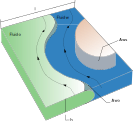
\includegraphics{figures/pdf/dessin_courbure.pdf}
\caption{Illustation of confined cocurrent two-phase flow between two
parallel plates and around cylinder obstacles.}\label{fig:modelStudy}
}
\end{figure}

Beside the interface curvature in the Hele-Shaw cell plane, the meniscus
in the perpendicular plane must be taken into account. Therefore, the
pressure jump at equilibrium across the interface reads

\[
\Delta p = \gamma \left(\frac{2}{h}+\kappa_{\parallel}\right),
\] \{\#eq:dP\}

where \(\gamma\) denotes the surface tension and \(\kappa_{\parallel}\)
the curvature in the Hele-Shaw plane
{[}\protect\hyperlink{ref-saffman1958penetration}{35}{]}. The
+\textbf{???} was completed in
{[}\protect\hyperlink{ref-park1984two}{36}{]} by an additional term that
pertains for dynamic film formation and a corrective \(\pi/4\) factor
for the curvature in the cell plane.

To compute the traction exerted by the fluids on the cell plates we need
to consider that the velocity profile in the \(z\)-direction is well
described by the Poiseuille flow profile,

\[
u=-\frac{1}{2\mu}\frac{dp}{dx}z(z-h).
\] \{\#eq:poiseuilleProfile\}

Then the friction force exerted on the bottom plate is given by

\[
\mu\frac{\partial u}{\partial z}\mid_{z=0}=-\frac{h}{2}\frac{dp}{dx}.
\] \{\#eq:poiseuilleFriction\}

Thus, the traction \(T_{i,pl}^x\) is obtained by multiplying the
friction force by two times the surface wetted by the fluid \(i\).

We can show that the average velocity taken over the interval between
the plates is written as follows

\[
\mathbf{U}(x,y,0)=-\frac{h^{2}}{12\mu}\nabla_{\parallel}p.
\] \{\#eq:darcyHeleShaw\}

There is therefore a direct analogy between flows in a 2D porous medium
and a flow in a Hele-Shaw cell, as can be seen in +\textbf{???}, where
the permeability is given by \(h^{2}/12\)
{[}\protect\hyperlink{ref-saffman1958penetration}{35}{]}.

\hypertarget{direct-numerical-simulations}{%
\section{Direct numerical
simulations}\label{direct-numerical-simulations}}

\hypertarget{equations}{%
\subsection{Equations}\label{equations}}

\hypertarget{level-set-model}{%
\subsubsection{Level Set model}\label{level-set-model}}

We use the Level Set method to capture the moving free interface between
the fluids. In this framework the fluid phases are identified with a
level set (scalar) function that goes smoothly from 0 to 1 across the
fluid interface and the interface is implicitely defined as the
iso-level \(\phi=0.5\). The transport of the level set function \(\phi\)
is governed by

\[
\frac{\partial\phi}{\partial t}+\nabla\cdot(\mathbf{u}\phi)=\tau\nabla\cdot\left(\psi\boldsymbol{\nabla}\phi-\phi(1-\phi)\frac{\boldsymbol{\nabla}\phi}{\vert\nabla\phi\vert}\right).
\] \{\#eq:advecphi\}

In this equation, \(\mathbf{u}\) is the velocity field, \(\tau\) and
\(\psi\) are two numerical parameters that control the diffuse interface
thickness and the amount of reinitialization of the \(\phi\) function,
respectively
{[}\protect\hyperlink{ref-Olsson2005}{37},\protect\hyperlink{ref-Olsson2007}{38}{]}.

\hypertarget{flow-model}{%
\subsubsection{Flow model}\label{flow-model}}

Remember that we need to take into account tangential stress as well
perpendicular stress due to the flow confinement, a full-3D resolution
of the flow equations would be meaningful. In order to avoid solving
such resource-intensive simulations we rather resolved 2D flow equations
plus an additional term taking into account the perpendicular stress.
The velocity and pressure fields are obtained by solving the 2D-modified
Stokes equations since the Reynolds number is assumed to be sufficiently
low so that the flow is creeping, the whole-domain formulation Stokes
and continuity equations read

\[
0=-\nabla p+\mu(\phi)\left(\nabla^{2}\mathbf{u}-k^{2}\mathbf{u}\right)+\mathbf{F}_{st},
\] \{\#eq:StokesMomentum\}

\[
0=\nabla\cdot\mathbf{u},
\] \{\#eq:StokesContinuity\}

where \(k=\frac{\sqrt{12}}{h}\) is an additional term that pertain to a
Darcy-term arising from the depth-averaging of the Stokes equation, as
described in the theoretical background section and \(\mathbf{F}_{st}\)
is the capillary contribution. The capillary contribution is difficult
to compute in volumetric methods such as Level Set and is itself the
object of a large body of work
{[}\protect\hyperlink{ref-Popinet2018}{39}{]}, this term is defined here
as

\[
\mathbf{F}_{st}=\gamma\kappa\delta(\phi)\mathbf{n},
\] \{\#eq:Fst\}

where \(\gamma\) is the surface tension, \(\kappa\) is the interface
mean curvature, \(\mathbf{n}\) denotes the unit normal to the interface
and \(\delta(\phi)\) is the Dirac delta function localized on the
interface {[}\protect\hyperlink{ref-Galusinski2008}{40}{]}. In this
framework the unit normal vector as well as the mean curvature are
obtained with the level set function \(\phi\) as

\[
\mathbf{n}=\frac{\boldsymbol{\nabla}\phi}{\vert\boldsymbol{\nabla}\phi\vert},
\]

\[
\kappa=\frac{\pi}{4}\nabla\cdot\left(\frac{\boldsymbol{\nabla}\phi}{\vert\boldsymbol{\nabla}\phi\vert}\right)+\kappa_{\perp},
\]

respectively, where the \(\pi/4\) correction was derived in
{[}\protect\hyperlink{ref-park1984two}{36}{]} and
\(\kappa_{\perp}=\frac{2}{h}\) is the out-of-plane curvature as
described previously in the theoretical background section.

The material parameters, that is the fluid density and the fluid
viscosity, varies smoothly from one fluid to another

\[
\rho(\phi)=\rho_{o}+(\rho_{w}-\rho_{o})\phi,
\]

\[
\mu(\phi)=\mu_{o}+(\mu_{w}-\mu_{o})\phi.
\]

\hypertarget{dimensionless-equations-and-relevant-dimensionless-numbers}{%
\subsubsection{Dimensionless equations and relevant dimensionless
numbers}\label{dimensionless-equations-and-relevant-dimensionless-numbers}}

If one define the following dimensionless variables

\[
\mathbf{u}=\mathbf{u}'\times U,\;p=p'\times\frac{\mu U}{l},\;\kappa=\kappa'\times l,\;\mathbf{x}=\mathbf{x}'\times l,
\]

where \(U\) is a reference velocity, \(\mu\) a reference viscosity and
\(l\) a reference length, Stokes and continuity equations can be recast
as

\[
0=-\nabla'p'+\frac{\mu(\phi)}{\mu}\nabla'^{2}\mathbf{u}'+\frac{\gamma}{\mu U}\kappa'\nabla'\phi,
\]

\[
0=\nabla'\cdot\mathbf{u}'.
\]

One can notice the two following dimensionless numbers

\[
\bar{\mu}=\frac{\mu(\phi)}{\mu},\;Ca^{-1}=\frac{\gamma}{\mu U},
\]

the viscosity ratio and the capillary number, respectively, which add up
to the already identified aspect ratio \(h/l\).

\hypertarget{test-case}{%
\subsection{Test case}\label{test-case}}

\hypertarget{geometry-and-boundary-conditions}{%
\subsubsection{Geometry and boundary
conditions}\label{geometry-and-boundary-conditions}}

We study a model system consisting of an array of cylinders in a thin
square cuboid, resembling a Hele-Shaw-cell with obstacles, as shown in
\cref{fig:model}. The two fluids are injected from the left at a
constant normal velocity. The outlet boundary condition for the flow is
a constant pressure. Initially the wetting fluid occupy the entire model
as depicted in \cref{fig:model}. The different boundary conditions are
listed in \cref{tbl:BC}.

\begin{figure}
\hypertarget{fig:model}{%
\centering
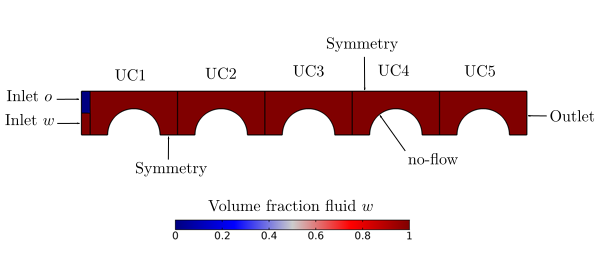
\includegraphics{figures/pdf/model.pdf}
\caption{The geometry used is an array of 5 cylinders in a thin square
cuboid, resembling a Hele-Shaw-cell where both fluids are injecting from
left to right, initially the square cuboïd are saturated with wetting
fluid (in blue), the length of one Unit-Cell (UC) is one
millimetre.}\label{fig:model}
}
\end{figure}

\begin{longtable}[]{@{}llll@{}}
\caption{Boundary conditions used. \label{tbl:BC}}\tabularnewline
\toprule
Boundary & u & p & \(\phi\)\tabularnewline
\midrule
\endfirsthead
\toprule
Boundary & u & p & \(\phi\)\tabularnewline
\midrule
\endhead
\(A_{ws}\) & 0 & - & \(\mathbf{n}\cdot\mathbf{u}\phi=0\)\tabularnewline
Outlet & - & 0 &
\(\mathbf{n}\cdot\boldsymbol{\nabla}\phi=0\)\tabularnewline
Inlet o & \(U_{o}^{x}=\mathrm{cst}\) & - & 0\tabularnewline
Inlet w & \(U_{w}^{x}=\mathrm{cst}\) & - & 1\tabularnewline
\bottomrule
\end{longtable}

\hypertarget{validation}{%
\subsubsection{Validation}\label{validation}}

\hypertarget{results}{%
\section{Results}\label{results}}

The results are given as a function of the dimensionless numbers defined
previously. The reference length \(l\) is the width of the unit cells
(0.5 mm), the reference viscosity is the invading fluid viscosity that
is two times greater (\(\mu_o=2\times 10^{-3}\) Pa.s) than the wetting
fluid viscosity. and the reference velocity is the total velocity, that
is \(U=U_{o}+U_{w}\). In consequence the capillary number and the
dimensionless inlet velocity read

\[
Ca=\frac{(U_{o}+U_{w})\mu_{o}}{\gamma},\;U_{w}^{'}=\frac{U_{w}}{U_{o}+U_{w}}=f_{f},\;U_{o}^{'}=1-f_{f},
\]

respectively, where \(f_{f}\) is the fractional flow. In the following
the viscosity ratio \(\bar{\mu}\) as well as the fractional flow
\(f_{f}\) are kept constant at 2 and 0.25, respectively.

In the following, the intrinsic permeability of the model is varied by
modifying the aperture between the two plates of the cell. We use five
different values for the aperture and the correspondence in terms of
intrinsic permeability is given in \cref{tbl:permeability} from
single-phase simulation. When \(h\rightarrow\infty\), it is expected
that the intrinsic permeability tends towards the permeability obtained
with purely 2D flow equations, this can be verified in
\cref{fig:permeability}. We obtain intrinsic permeability values typical
of high permeability porous media with the selected aperture values.

\begin{longtable}[]{@{}lll@{}}
\caption{Equivalence between the value of the cell plates aperture and
the intrinsic permeability of the model obtained either from the
intrinsic permeability for flow between two plates or from single-phase
simulation in our model. \label{tbl:permeability}}\tabularnewline
\toprule
\(l/h\) & \(h^2/12\) (darcy) & \(k\) Simulation (darcy)\tabularnewline
\midrule
\endfirsthead
\toprule
\(l/h\) & \(h^2/12\) (darcy) & \(k\) Simulation (darcy)\tabularnewline
\midrule
\endhead
0.2 & \(5.21 \times 10^{5}\) & \(1.48 \times 10^{4}\)\tabularnewline
2.0 & \(5.21 \times 10^{3}\) & \(2.85 \times 10^{3}\)\tabularnewline
4.0 & \(1.30 \times 10^{3}\) & \(8.63 \times 10^{2}\)\tabularnewline
8.0 & \(3.26 \times 10^{2}\) & \(2.35 \times 10^{2}\)\tabularnewline
20 & \(5.21 \times 10^{1}\) & \(3.94 \times 10^{1}\)\tabularnewline
\bottomrule
\end{longtable}

\begin{figure}
\hypertarget{fig:permeability}{%
\centering
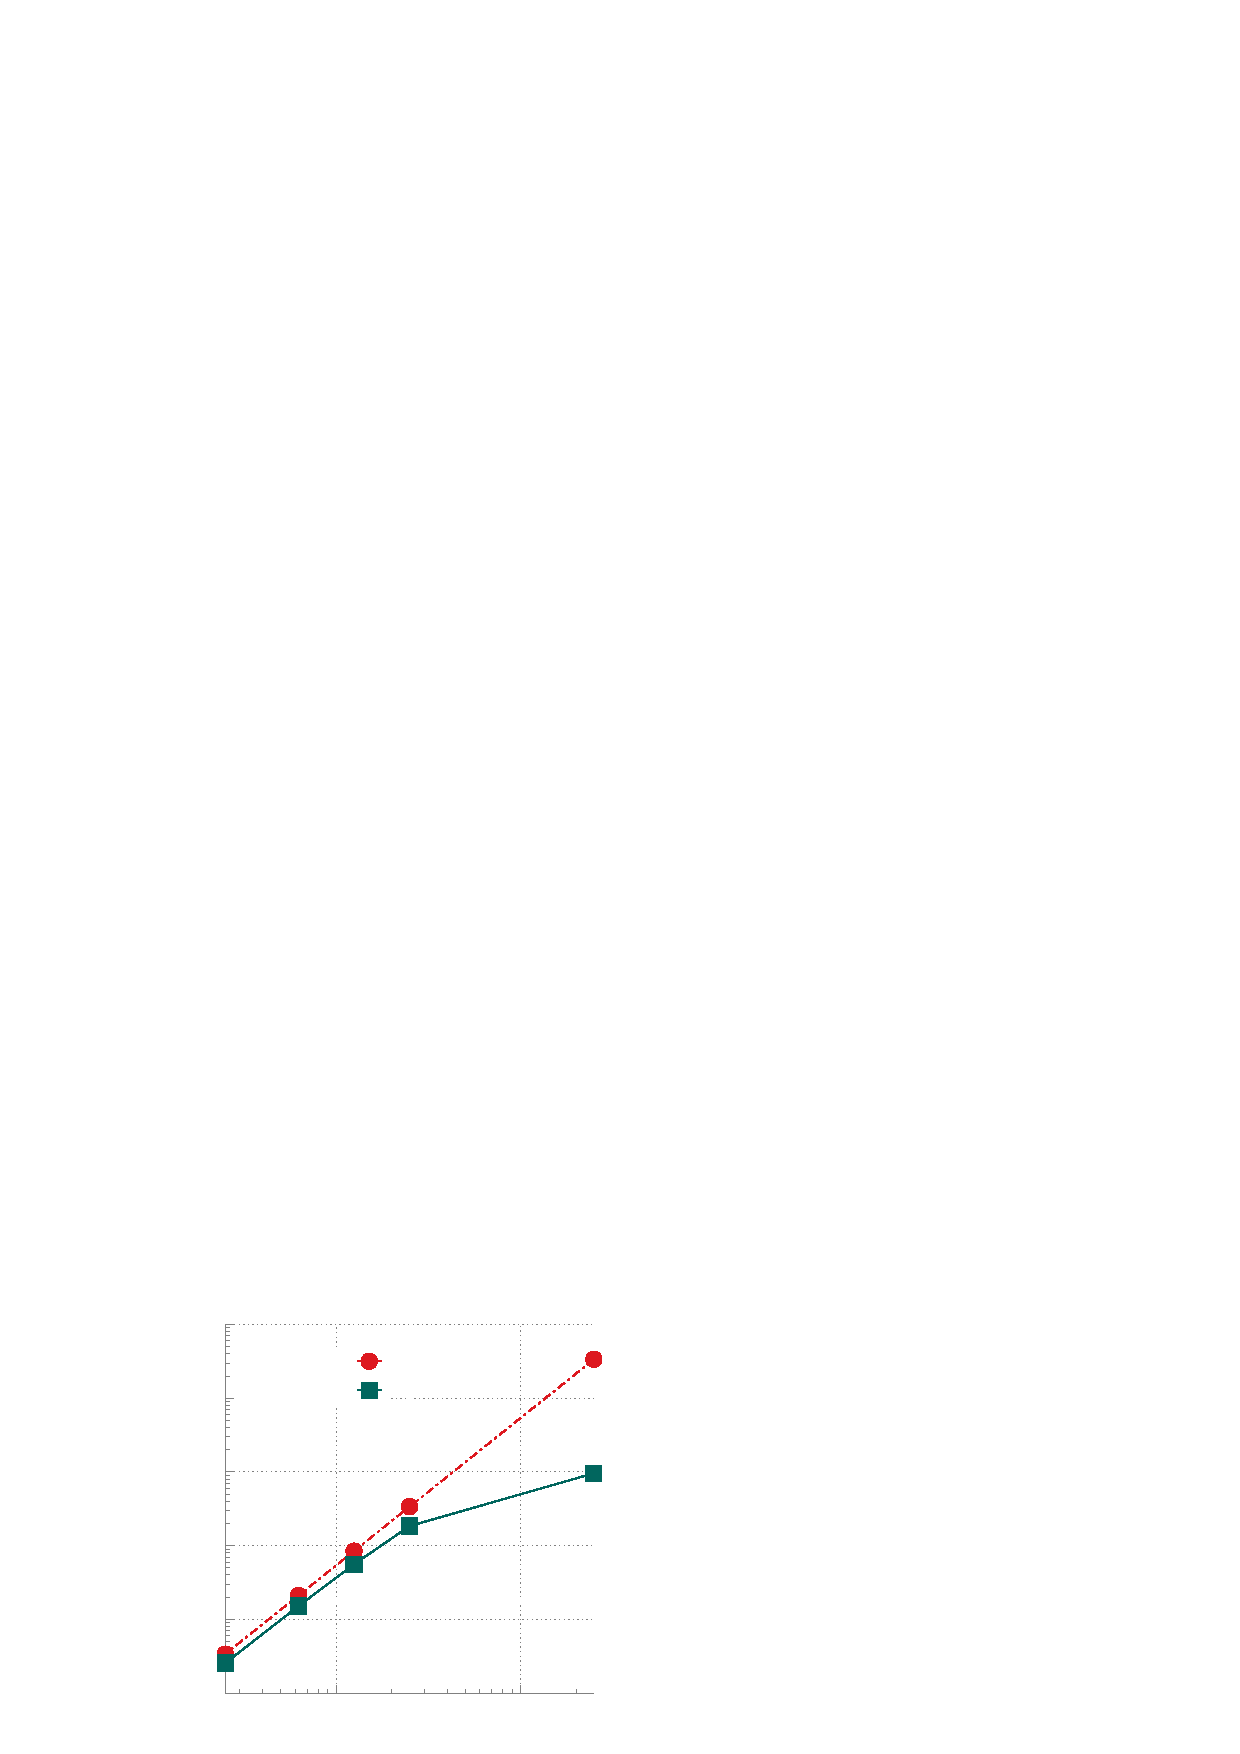
\includegraphics{figures/pdf/permeability.pdf}
\caption{Intrinsic permeability of the Hele-Shaw cell normalized by the
intrinsic permeability obtained from pure 2D
simulation.}\label{fig:permeability}
}
\end{figure}

\hypertarget{wetting-fluid-saturation-decreases-when-permeability-is-decreasing}{%
\subsection{Wetting fluid saturation decreases when permeability is
decreasing}\label{wetting-fluid-saturation-decreases-when-permeability-is-decreasing}}

Before we turn to the study of traction terms it is worth invesigate the
effect of varying permeability on the fluid repartition and the velocity
fields. Wetting fluid saturation in the third unit-cell (UC3), computed
accordingly to +\textbf{???}, is given as a function of the
dimensionless aperture between the plates in \cref{fig:saturation}.

The wetting fluid saturation non-linearly decreases with \(h^*\) and
stays at moderate values, between 0.6 and 0.3. A smaller capillary
number tends to slightly increase the wetting fluid saturation at
steady-state.

\begin{figure}
\hypertarget{fig:saturation}{%
\centering
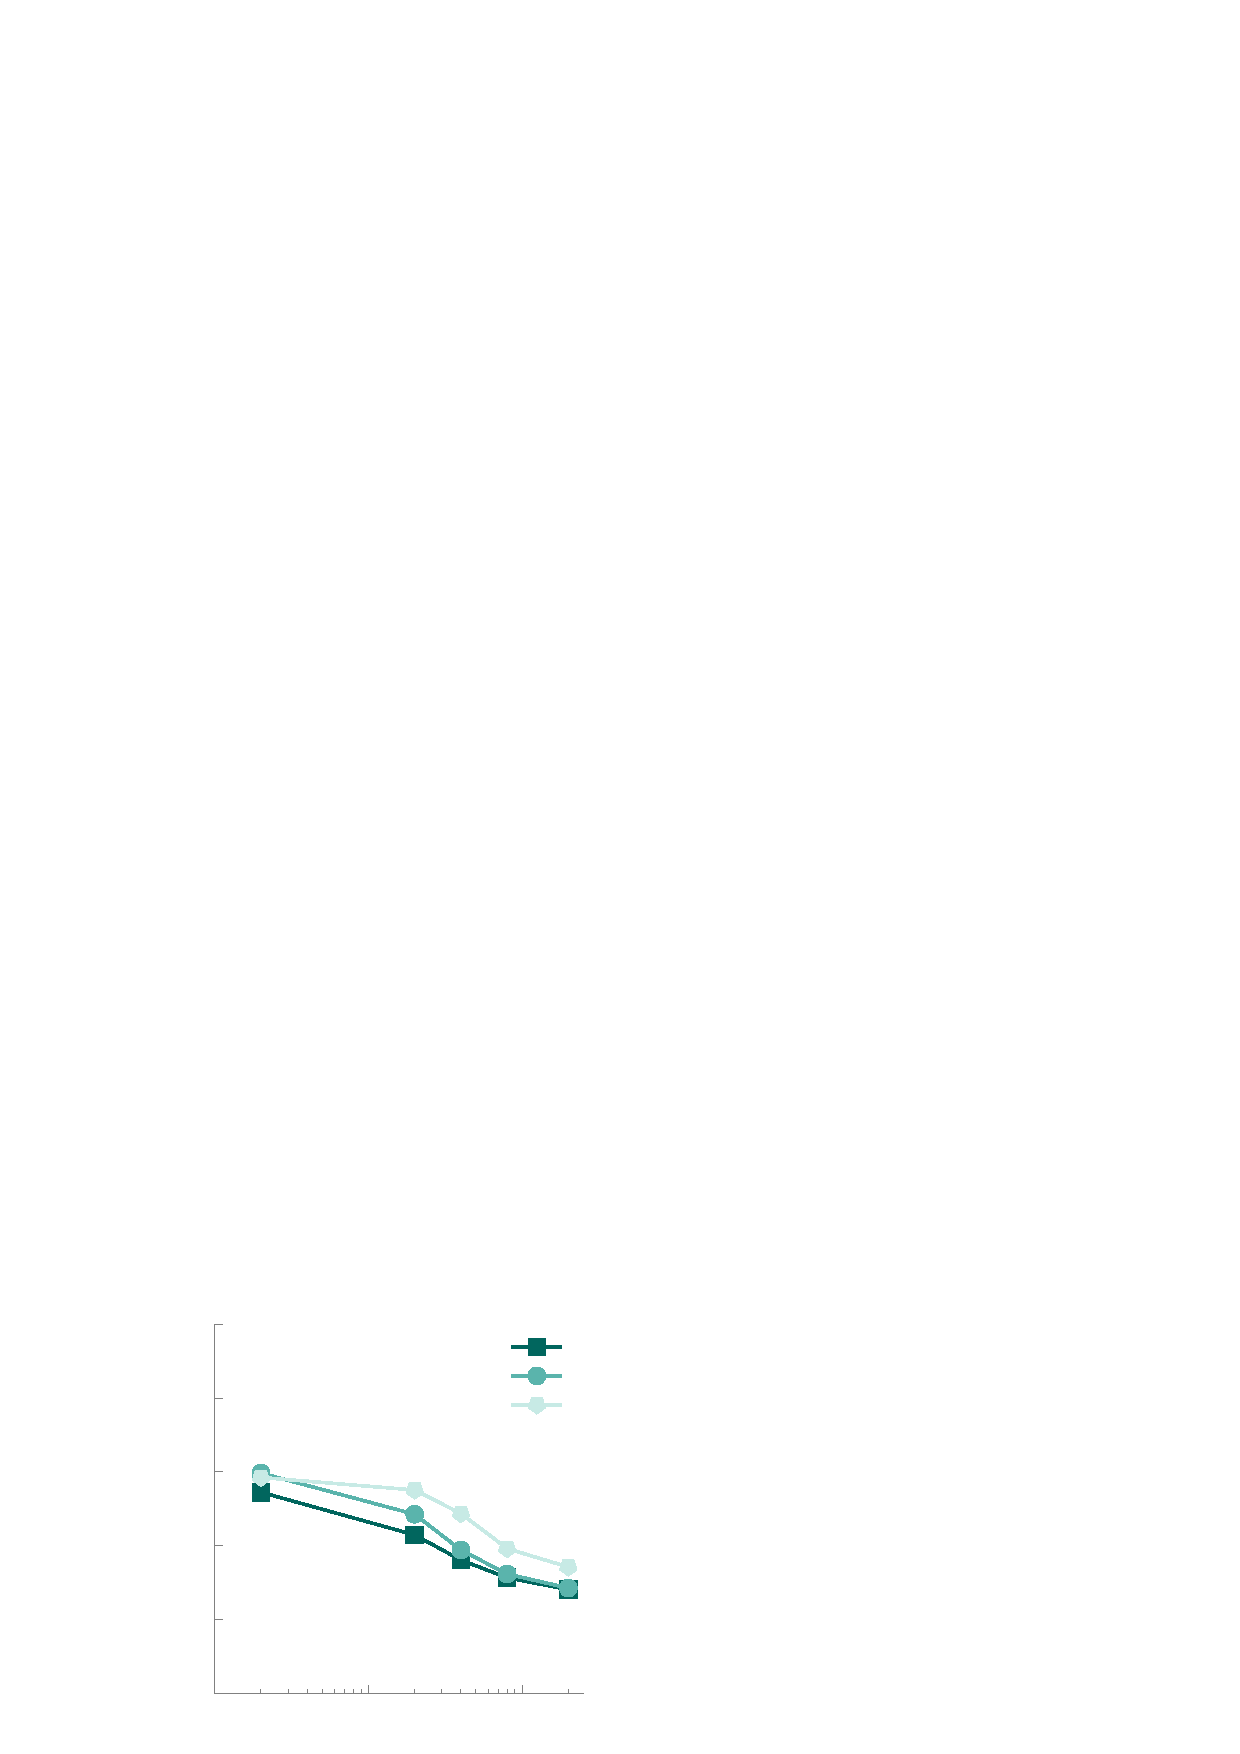
\includegraphics{figures/pdf/saturation.pdf}
\caption{Saturation in wetting fluid as a function of the dimensionless
aperture \(h^{*}=h/l\) and for different values of the capillary number
(UC3) at steady-state.}\label{fig:saturation}
}
\end{figure}

Let us take a closer look at the interface position for different values
of \(h^*\) for \(Ca=1\) and \(Ca=0.05\) in \cref{fig:interfaceCa1} and
\cref{fig:interfaceCa005}, respectively. The interface for small
capillary number and large aperture is significantly flatter than for
high capillary number and/or small aperture. One also noted that the
interface is symmetrical when the capillary number is large whereas it
loses this property for a smaller capillary number and for larger
aperture between the plates. On the same plots we show the position of
the interface in a purely 2D case, and one can see that it is very close
to the solution for \(1/h^*=0.2\). The fluid-fluid interface moves
closer to the cylinder for decreasing aperture (i.e.~intrinsic
permeability), this has an impact on the velocity fields, as shown in
\cref{fig:UvelocityCa1LH2} and \cref{fig:UvelocityCa1LH20}, which
represent the dimensionless \(x\)-component of the velocity for
\(Ca=1.0\) and \(1/h^*=2\) and \(1/h^*=20\), respectively. Clearly, what
is happening here is that the velocity profile is close to the
Poiseuille profile as long as the interface is not too close from the
solid. To verify this, we plot in \cref{fig:uprofileCa1} the
dimensionless \(x\)-component of the velocity along the line shown in
\cref{fig:UvelocityCa1LH20}. The profile for the pure 2D solution
(\(h\rightarrow\infty\)) resembles a Poiseuille profile while for
decreasing aperture the maximum velocity is observed between the solid
and the fluid-fluid interface.

\begin{figure}
\hypertarget{fig:interfaceCa1}{%
\centering
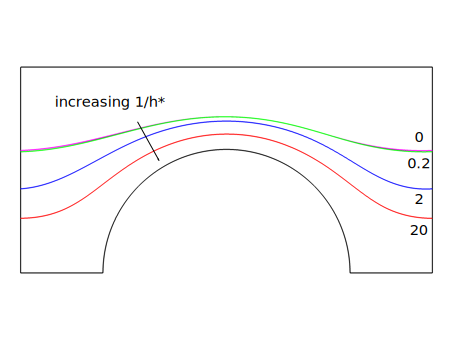
\includegraphics{figures/pdf/interfaceCa1.pdf}
\caption{Interface position at steady-state in UC3 for
\(Ca=5\times10^{-2}\).}\label{fig:interfaceCa1}
}
\end{figure}

\begin{figure}
\hypertarget{fig:interfaceCa005}{%
\centering
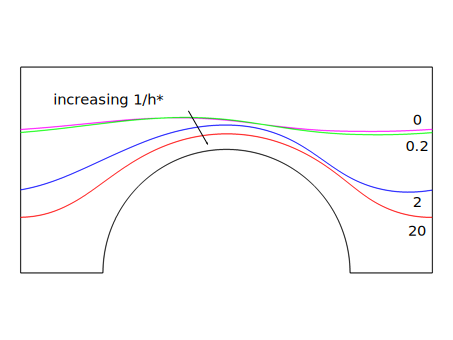
\includegraphics{figures/pdf/interfaceCa005.pdf}
\caption{Interface position at steady-state in UC3 for
\(Ca=5\times10^{-2}\).}\label{fig:interfaceCa005}
}
\end{figure}

\begin{figure}
\hypertarget{fig:UvelocityCa1LH2}{%
\centering
\includegraphics{figures/png/Uvelocity_Ca1LH2.png}
\caption{Dimensionless \(x\)-component of the velocity in UC3 for
\(Ca=1\) and \(1/h^*=2\).}\label{fig:UvelocityCa1LH2}
}
\end{figure}

\begin{figure}
\hypertarget{fig:UvelocityCa1LH20}{%
\centering
\includegraphics{figures/png/Uvelocity_Ca1LH20.png}
\caption{Dimensionless \(x\)-component of the velocity in UC3 for
\(Ca=1\) and \(1/h^*=20\).}\label{fig:UvelocityCa1LH20}
}
\end{figure}

\begin{figure}
\hypertarget{fig:uprofileCa1}{%
\centering
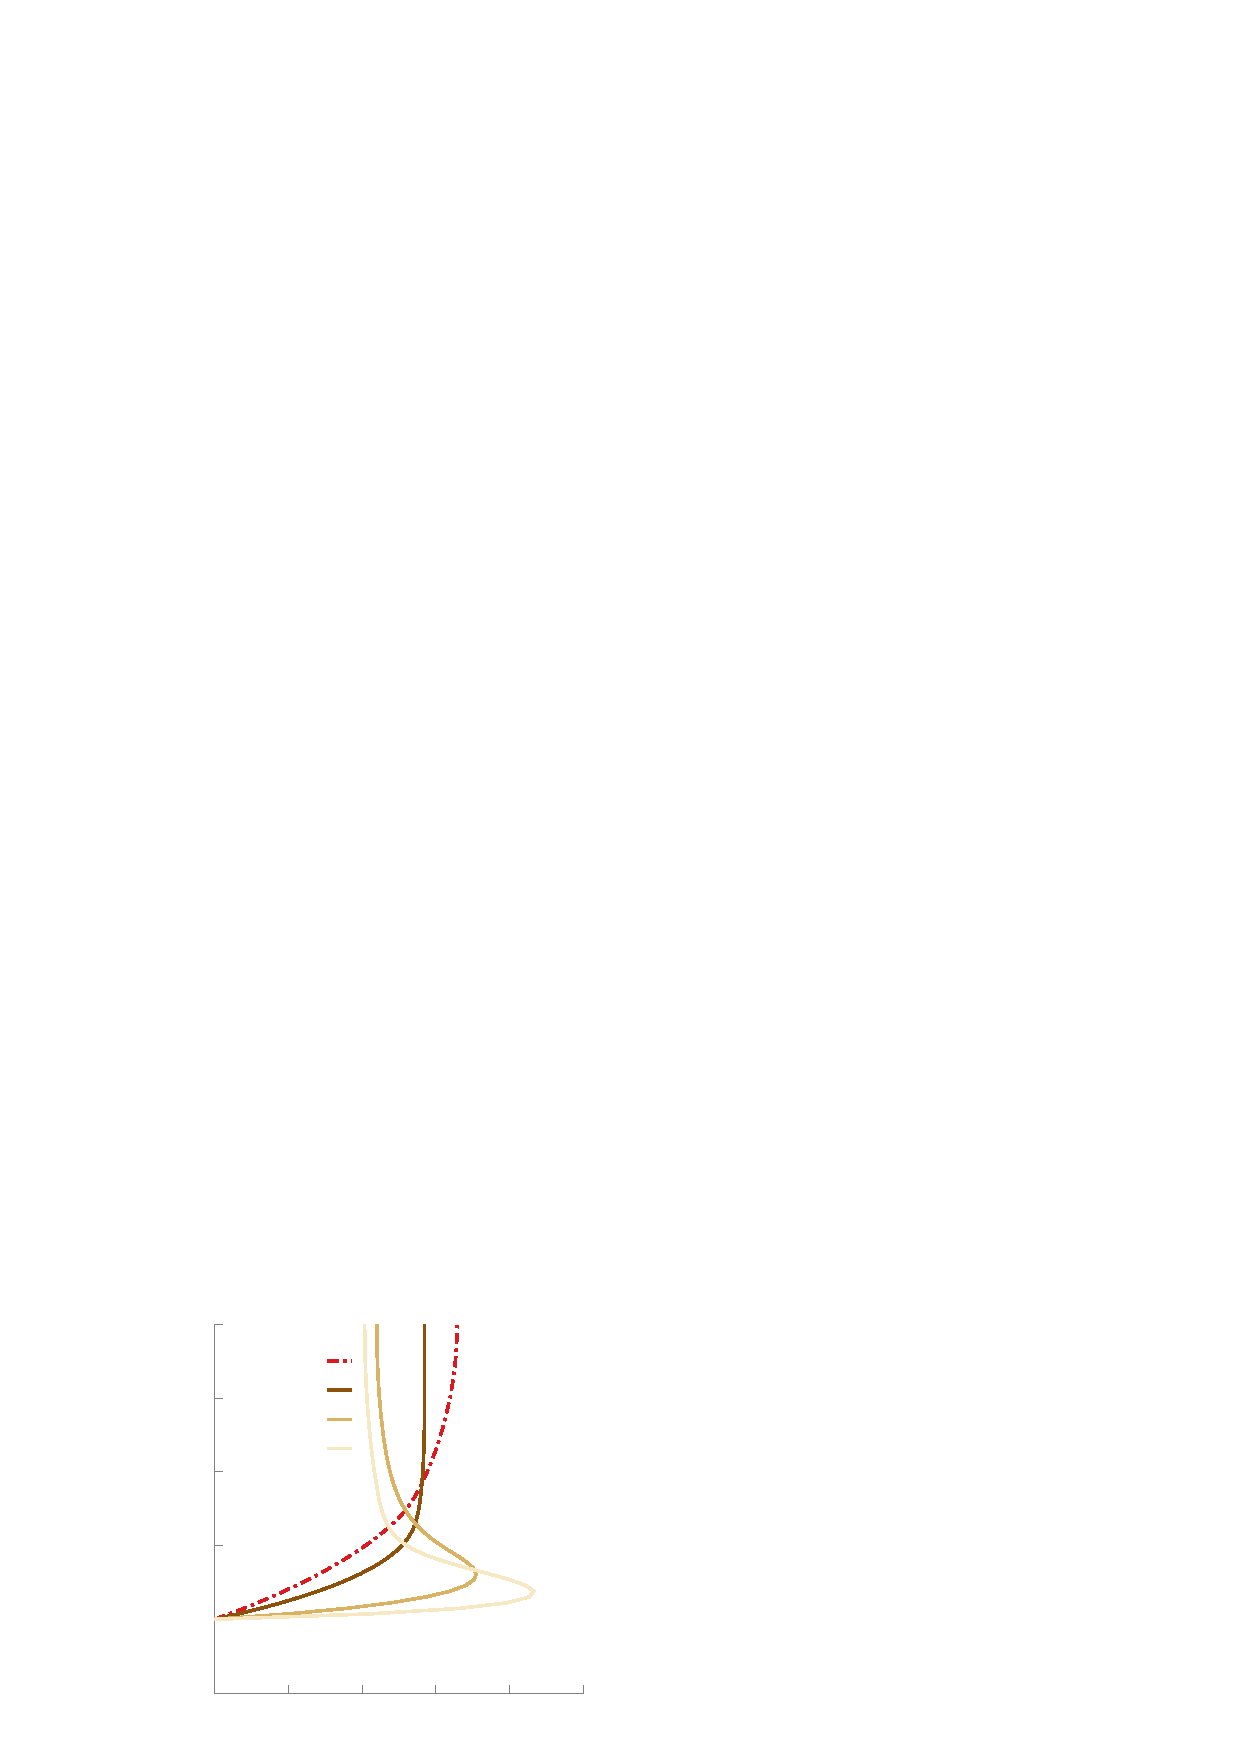
\includegraphics{figures/pdf/uprofileCa1.pdf}
\caption{Dimensionless \(x\)-velocity profile in UC3 for \(Ca=1\) and
different values of the intrinsic permeability.}\label{fig:uprofileCa1}
}
\end{figure}

\hypertarget{dynamic-capillary-pressure-scale-linearly-with-the-gap-between-hele-shaw-plates-regardless-of-the-capillary-number}{%
\subsection{Dynamic capillary pressure scale linearly with the gap
between Hele-Shaw plates regardless of the capillary
number}\label{dynamic-capillary-pressure-scale-linearly-with-the-gap-between-hele-shaw-plates-regardless-of-the-capillary-number}}

We now consider the dynamic capillary pressure as defined in
+\textbf{???} as a function of \(h^*\). As can be seen on \cref{fig:Pc},
\(P_c\) perfectly scales linearly with \(h^*\), regardless of the
capillary number. One can find on the same plot the theoretical pressure
jump across the fluid-fluid interface due to the out-of-plane meniscus.
This pressure jump closely matches the computed dynamic capillary
pressure and to this point, we can conclude that even for the largest
aperture the difference of mean intrinsic pressure is given by the
meniscus between the two plates. Seeing this, it is worthwhile to
contrast the pressure jump across the interface with the pressure
gradient across the cell. We plot the pressure field and pressure
contour in the third unit-cell (UC3) for \(Ca=1\) and \(1/h^*=2\) on
\cref{fig:pFieldCa1} (a) and \(1/h^*=20\) on \cref{fig:pFieldCa1} (b).
One can note that, although the pressure jump is greater in absolute
terms, it is almost unobservable for the smallest aperture because of
the large pressure gradient.

\begin{figure}
\hypertarget{fig:Pc}{%
\centering
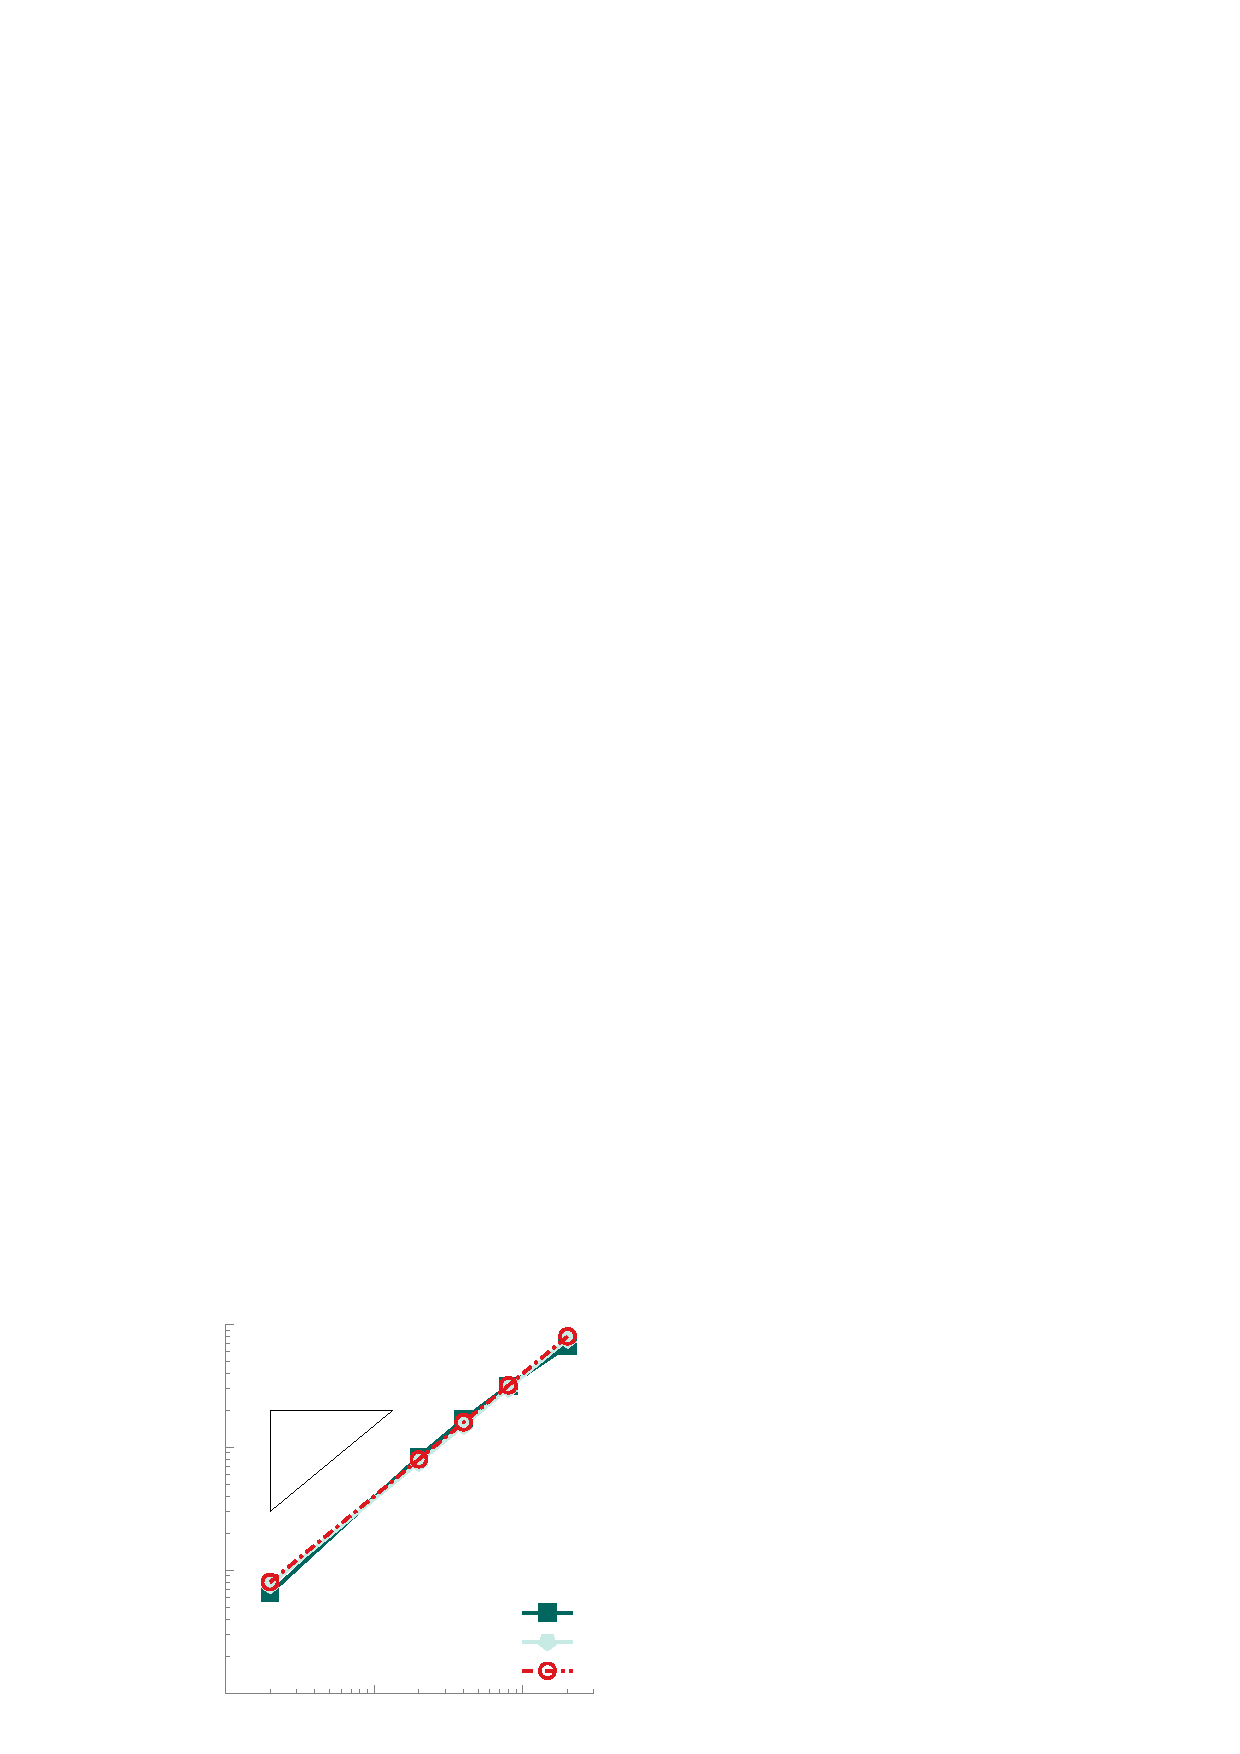
\includegraphics{figures/pdf/Pc.pdf}
\caption{Dynamic capillary pressure in UC3 as a function of \(h^*\) for
different capillary numbers and pressure drop across the fluid-fluid
based on the out-of-plane meniscus at steady-state}\label{fig:Pc}
}
\end{figure}

\begin{figure}
\hypertarget{fig:pFieldCa1}{%
\centering
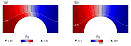
\includegraphics{figures/pdf/pFieldCa1.pdf}
\caption{Pressure field in UC3 for \(Ca=1\) and (a) \(1/h^*=2\) and (b)
\(1/h^*=20\) and interface position as the iso-\(\phi\)=0.5
contour}\label{fig:pFieldCa1}
}
\end{figure}

\begin{figure}
\hypertarget{fig:pFieldCa001}{%
\centering
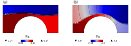
\includegraphics{figures/pdf/pFieldCa001.pdf}
\caption{Pressure field in UC3 for \(Ca=1 \times 10^{-2}\) and (a)
\(1/h^*=2\) and (b) \(1/h^*=20\) and interface position as the
iso-\(\phi\)=0.5 contour}\label{fig:pFieldCa001}
}
\end{figure}

\hypertarget{fluid-fluid-traction-increases-faster-compared-to-solid-fluid-traction-when-permeability-is-decreasing}{%
\subsection{Fluid-fluid traction increases faster compared to
solid-fluid traction when permeability is
decreasing}\label{fluid-fluid-traction-increases-faster-compared-to-solid-fluid-traction-when-permeability-is-decreasing}}

Here we plot traction terms as a function of the aperture between the
Hele-Shaw plates. We first plot on \cref{fig:drag_plates} traction
exerted on the Hele-Shaw plates by each fluid, remember that this term
is computed as described in the theoretical background section.
Logically, the traction exerted by the non-wetting fluid on the cell
plates becomes more important for smaller aperture since, as discussed
above, the surface wetted by this fluid becomes larger as the aperture
decreases.

\begin{figure}
\hypertarget{fig:drag_plates}{%
\centering
\includegraphics{figures/pdf/drag_plates.pdf}
\caption{\(x\)-component of the traction on Hele-Shaw cell plates by
each fluid in UC3, as a function of the dimensionless gap and for
different capillary numbers at steady-state.}\label{fig:drag_plates}
}
\end{figure}

In \cref{fig:drag_solid} we plot the sum of traction (\(x\)-component)
exerted on all solid-fluid boundaries as a function of the dimensionless
aperture between the plates and for different capillary numbers. For
\(1/h^*\) greater than 2, the traction scale a bit slower than
\(1/h^2\). Logically, the greater the capillary number, the greater the
traction term.

\begin{figure}
\hypertarget{fig:drag_solid}{%
\centering
\includegraphics{figures/pdf/drag_solid.pdf}
\caption{\(x\)-component of the traction exerted on the solid-fluid
boundaries in UC3 as a function of the dimensionless aperture and for
different capillary numbers at steady-state.}\label{fig:drag_solid}
}
\end{figure}

We compute the fluid-fluid traction \(T_{ij}\) in two steps. The first
step concerns the viscous part of the stress tensor, which is calculated
directly from the velocity gradients available on the interface contour.
The second step concerns the pressure part, which is obtained by
applying the divergence theorem on each phase into UC3. In
\cref{fig:drag_fluidint} we plot the traction on the fluid-fluid
interface \(T_{ow}\) as a function of \(h^*\). From \(1/h^*=2\) the
traction scale a bit faster than \(1/h^2\).

\begin{figure}
\hypertarget{fig:drag_fluidint}{%
\centering
\includegraphics{figures/pdf/drag_fluidint.pdf}
\caption{\(x\)-component of the traction exerted on the fluid-fluid
interface in UC3 as a function of the dimensionless aperture and for
different capillary numbers at steady-state.}\label{fig:drag_fluidint}
}
\end{figure}

\hypertarget{decreasing-the-permeability-does-not-imply-that-the-share-of-the-fluid-fluid-traction-is-negligible-in-the-total-traction}{%
\subsection{Decreasing the permeability does not imply that the share of
the fluid-fluid traction is negligible in the total
traction}\label{decreasing-the-permeability-does-not-imply-that-the-share-of-the-fluid-fluid-traction-is-negligible-in-the-total-traction}}

Let us now sum up all the traction terms and answer the question of the
share of traction exerted on the fluid-fluid boundaries in total
traction. The ratio \(T_{int}^x/T_{s}^x\), were \(s={pl+cyl}\) and
\(int={wo+ow}\), is given as a function of the dimensionless aperture
between the Hele-Shaw plates in \cref{fig:ratioDrag}. The traction
exerted on the fluid-fluid boundary reaches between 10 to 50\% of the
traction exerted on the solid-fluid boundaries. Interestingly, the ratio
varies non-monotonically with \(h^*\), the minimum is reached for the
smallest capillary numbers and for a medium range of the aperture
values.

As the capillary number decreases, variations with the aperture are
amplified. Thus, it is for the lowest capillary number tested that we
obtain both the maximum and minimum values of the ratio
\(T_{int}^x/T_{s}^x\).

\begin{figure}
\hypertarget{fig:ratioDrag}{%
\centering
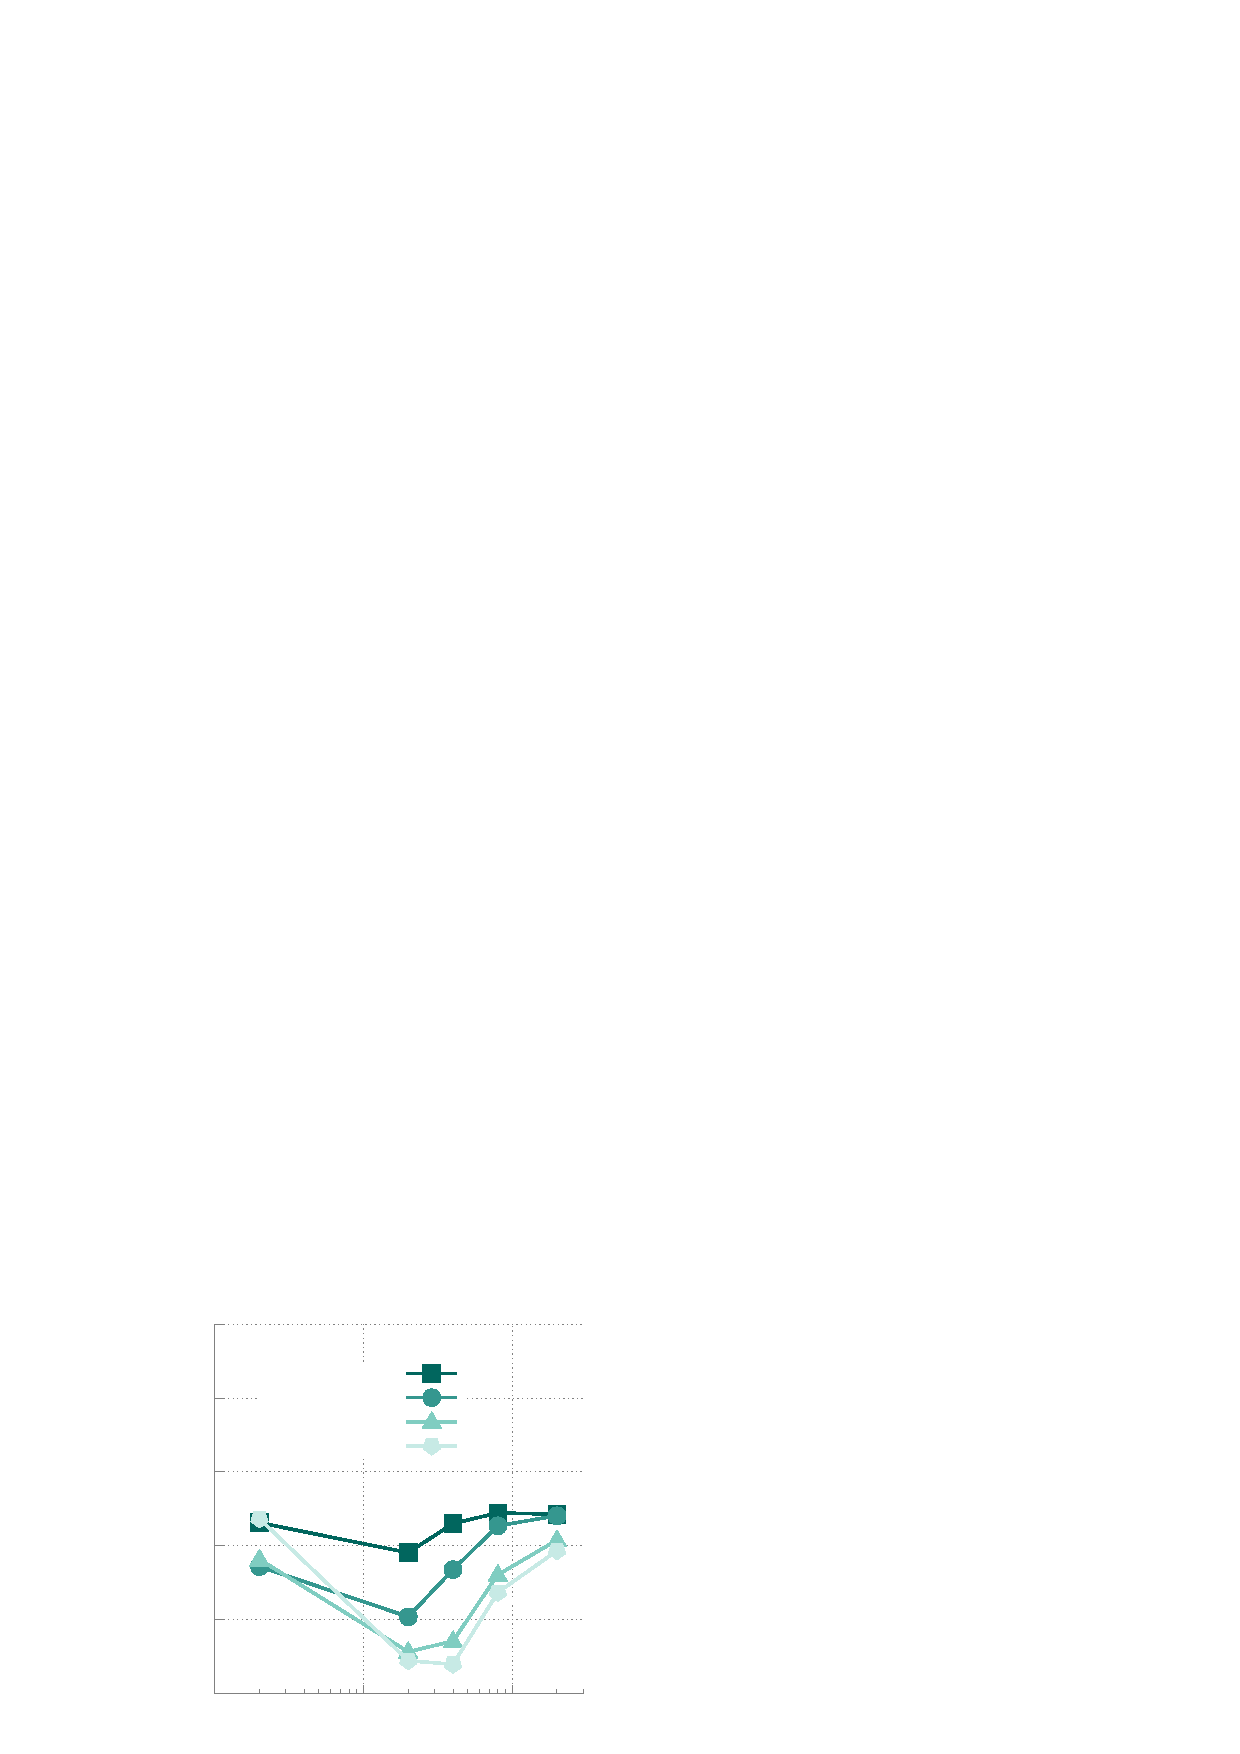
\includegraphics{figures/pdf/ratioDrag.pdf}
\caption{Ratio of traction on fluid-fluid interface over traction on
solid-fluid interfaces in UC3 as a function of the dimensionless
aperture between the Hele-Shaw plates and for different capillary
numbers at steady-state.}\label{fig:ratioDrag}
}
\end{figure}

\hypertarget{conclusion}{%
\section{Conclusion}\label{conclusion}}

In this work, we investigated the effect of varied permeability on
cocurrent two-phase flow in a Hele-Shaw cell. We focused on the value of
the traction terms, that are necessary to close the macroscopic flow
equations. The idea of solving modified 2D-Stokes equations with a
supplementary Darcy term allowed us to modify the intrinsic permeability
of the structure without having to modify the geometry per se. The
chosen range for intrinsic permeability values is typical of
high-permeability porous media, for which it is known that the flow
regimes are characterized by the large extent of the fluid-fluid
interface the fluids (e.g.~film flow). Through direct numerical
simulation and a Level Set method to handle the free interface between
the fluid we have found that

\hypertarget{references}{%
\section*{References}\label{references}}
\addcontentsline{toc}{section}{References}

\hypertarget{refs}{}
\leavevmode\hypertarget{ref-fetter2017contaminant}{}%
{[}1{]} Fetter CW, Boving T, Kreamer D. Contaminant hydrogeology.
Waveland Press; 2017.

\leavevmode\hypertarget{ref-clavier2017modeling}{}%
{[}2{]} Clavier R, Chikhi N, Fichot F, Quintard M. Modeling of inertial
multi-phase flows through high permeability porous media: Friction
closure laws. International Journal of Multiphase Flow 2017;91:243--61.

\leavevmode\hypertarget{ref-Santos1991}{}%
{[}3{]} Santos JM de, Melli TR, Scriven LE. Mechanics of gas-liquid flow
in packed-bed contactors. Annual Review of Fluid Mechanics
1991;23:233--60.
\url{https://doi.org/10.1146/annurev.fl.23.010191.001313}.

\leavevmode\hypertarget{ref-davit2018one}{}%
{[}4{]} Davit Y, Quintard M. One-phase and two-phase flow in highly
permeable porous media. Heat Transfer Engineering 2018:1--19.

\leavevmode\hypertarget{ref-dullien2012porous}{}%
{[}5{]} Dullien FAL. Porous media: Fluid transport and pore structure.
Academic press; 2012.

\leavevmode\hypertarget{ref-Avraam1995a}{}%
{[}6{]} Avraam DG, Payatakes AC. Flow regimes and relative
permeabilities during steady-state two-phase flow in porous media.
Journal of Fluid Mechanics 1995;293:207--36.
\url{https://doi.org/10.1017/S0022112095001698}.

\leavevmode\hypertarget{ref-armstrong2016beyond}{}%
{[}7{]} Armstrong RT, McClure JE, Berrill MA, Rücker M, Schlüter S, Berg
S. Beyond darcy's law: The role of phase topology and ganglion dynamics
for two-fluid flow. Physical Review E 2016;94:043113.

\leavevmode\hypertarget{ref-wyckoff1936flow}{}%
{[}8{]} Wyckoff RD, Botset HG. The flow of gas-liquid mixtures through
unconsolidated sands. Physics 1936;7:325--45.

\leavevmode\hypertarget{ref-muskat1938flow}{}%
{[}9{]} Muskat M. The flow of homogeneous fluids through porous media.
Soil Science 1938;46:169.

\leavevmode\hypertarget{ref-leverett1941capillary}{}%
{[}10{]} Leverett M, others. Capillary behavior in porous solids.
Transactions of the AIME 1941;142:152--69.

\leavevmode\hypertarget{ref-kalaydjian1992dynamic}{}%
{[}11{]} Kalaydjian F-M, others. Dynamic capillary pressure curve for
water/oil displacement in porous media: Theory vs. Experiment. In:. SPE
annual technical conference and exhibition, Society of Petroleum
Engineers; 1992.

\leavevmode\hypertarget{ref-Hassanizadeh1993}{}%
{[}12{]} Hassanizadeh SM, Gray WG. Thermodynamic basis of capillary
pressure in porous media. Water Resources Research 1993;29:3389--405.
\url{https://doi.org/10.1029/93WR01495}.

\leavevmode\hypertarget{ref-barenblatt2003mathematical}{}%
{[}13{]} Barenblatt GI, Patzek TW, Silin DB. The mathematical model of
nonequilibrium effects in water-oil displacement. SPE Journal
2003;8:409--16.

\leavevmode\hypertarget{ref-hilfer1998macroscopic}{}%
{[}14{]} Hilfer R. Macroscopic equations of motion for two-phase flow in
porous media. Physical Review E 1998;58:2090.

\leavevmode\hypertarget{ref-blunt2017multiphase}{}%
{[}15{]} Blunt MJ. Multiphase flow in permeable media: A pore-scale
perspective. Cambridge University Press; 2017.

\leavevmode\hypertarget{ref-MARLE1982643}{}%
{[}16{]} Marle CM. On macroscopic equations governing multiphase flow
with diffusion and chemical reactions in porous media. International
Journal of Engineering Science 1982;20:643--62.
\url{https://doi.org/https://doi.org/10.1016/0020-7225(82)90118-5}.

\leavevmode\hypertarget{ref-Whitaker1986a}{}%
{[}17{]} Whitaker S. Flow in porous media II: The governing equations
for immiscible, two-phase flow. Transport in Porous Media
1986;1:105--25.

\leavevmode\hypertarget{ref-auriault1986remarques}{}%
{[}18{]} Auriault J, Sanchez-Palencia E. Remarques sur la loi de darcy
pour les écoulements biphasiques en milieu poreux. Journal of
Theoretical and Applied Mechanics, Numéro Spécial 1986:p141--156.

\leavevmode\hypertarget{ref-kalaydjian1990origin}{}%
{[}19{]} Kalaydjian F. Origin and quantification of coupling between
relative permeabilities for two-phase flows in porous media. Transport
in Porous Media 1990;5:215--29.

\leavevmode\hypertarget{ref-Lasseux1996}{}%
{[}20{]} Lasseux D, Quintard M, Whitaker S. Determination of
permeability tensors for two-phase flow in homogeneous porous media:
Theory. Transport in Porous Media 1996;24:107--37.

\leavevmode\hypertarget{ref-zarcone1994determination}{}%
{[}21{]} Zarcone C, Lenormand R. Détermination expérimentale du couplage
visqueux dans les écoulements diphasiques en milieu poreux. Comptes
Rendus de L'Académie Des Sciences Série II, Mécanique, Physique, Chimie,
Astronomie 1994;318:1429--35.

\leavevmode\hypertarget{ref-Dullien1996}{}%
{[}22{]} Dullien FAL, Dong M. Experimental determination of the flow
transport coefficients in the coupled equations of two-phase flow in
porous media. Transport in Porous Media 1996;25:97--120.
\url{https://doi.org/10.1007/bf00141264}.

\leavevmode\hypertarget{ref-ramakrishnan2015measurement}{}%
{[}23{]} Ramakrishnan TS, Goode PA. Measurement of off-diagonal
transport coefficients in two-phase flow in porous media. Journal of
Colloid and Interface Science 2015;449:392--8.

\leavevmode\hypertarget{ref-Rose1988}{}%
{[}24{]} Rose W. Measuring transport coefficients necessary for the
description of coupled two-phase flow of immiscible fluids in porous
media. Transport in Porous Media 1988;3:163--71.
\url{https://doi.org/10.1007/BF00820343}.

\leavevmode\hypertarget{ref-bentsen1993use}{}%
{[}25{]} Bentsen RG, Manai AA. On the use of conventional cocurrent and
countercurrent effective permeabilities to estimate the four generalized
permeability coefficients which arise in coupled, two-phase flow.
Transport in Porous Media 1993;11:243--62.

\leavevmode\hypertarget{ref-langaas2001numerical}{}%
{[}26{]} Langaas K, Papatzacos P. Numerical investigations of the steady
state relative permeability of a simplified porous medium. Transport in
Porous Media 2001;45:241--66.

\leavevmode\hypertarget{ref-Avraam1995}{}%
{[}27{]} Avraam DG, Payatakes AC. Generalized relative permeability
coefficients during steady-state two-phase flow in porous media, and
correlation with the flow mechanisms. Transport in Porous Media
1995;20:135--68. \url{https://doi.org/10.1007/bf00616928}.

\leavevmode\hypertarget{ref-Rothman1990}{}%
{[}28{]} Rothman DH. Macroscopic laws for immiscible two-phase flow in
porous media: Results from numerical experiments. Journal of Geophysical
Research 1990;95:8663. \url{https://doi.org/10.1029/jb095ib06p08663}.

\leavevmode\hypertarget{ref-Li2005}{}%
{[}29{]} Li H, Pan C, Miller CT. Pore-scale investigation of viscous
coupling effects for two-phase flow in porous media. Physical Review E
2005;72. \url{https://doi.org/10.1103/physreve.72.026705}.

\leavevmode\hypertarget{ref-Yiotis2007}{}%
{[}30{]} Yiotis AG, Psihogios J, Kainourgiakis ME, Papaioannou A, Stubos
AK. A lattice boltzmann study of viscous coupling effects in immiscible
two-phase flow in porous media. Colloids and Surfaces A: Physicochemical
and Engineering Aspects 2007;300:35--49.
\url{https://doi.org/https://doi.org/10.1016/j.colsurfa.2006.12.045}.

\leavevmode\hypertarget{ref-odeh1959effect}{}%
{[}31{]} Odeh AS, others. Effect of viscosity ratio on relative
permeability (includes associated paper 1496-g) 1959.

\leavevmode\hypertarget{ref-shams2018study}{}%
{[}32{]} Shams M, Raeini AQ, Blunt MJ, Bijeljic B. A study to
investigate viscous coupling effects on the hydraulic conductance of
fluid layers in two-phase flow at the pore level. Journal of Colloid and
Interface Science 2018;522:299--310.

\leavevmode\hypertarget{ref-Whitaker2013}{}%
{[}33{]} Whitaker S. The method of volume averaging. vol. 13. Springer
Science \& Business Media; 2013.

\leavevmode\hypertarget{ref-Kalaydjian1987}{}%
{[}34{]} Kalaydjian F. A macroscopic description of multiphase flow in
porous media involving spacetime evolution of fluid/fluid interface.
Transport in Porous Media 1987;2:537--52.
\url{https://doi.org/10.1007/BF00192154}.

\leavevmode\hypertarget{ref-saffman1958penetration}{}%
{[}35{]} Saffman PG, Taylor GI. The penetration of a fluid into a porous
medium or hele-shaw cell containing a more viscous liquid. Proceedings
of the Royal Society of London Series A Mathematical and Physical
Sciences 1958;245:312--29.

\leavevmode\hypertarget{ref-park1984two}{}%
{[}36{]} Park C-W, Homsy G. Two-phase displacement in hele shaw cells:
Theory. Journal of Fluid Mechanics 1984;139:291--308.

\leavevmode\hypertarget{ref-Olsson2005}{}%
{[}37{]} Olsson E, Kreiss G. A conservative level set method for two
phase flow. Journal of Computational Physics 2005;210:225--46.
\url{https://doi.org/https://doi.org/10.1016/j.jcp.2005.04.007}.

\leavevmode\hypertarget{ref-Olsson2007}{}%
{[}38{]} Olsson E, Kreiss G, Zahedi S. A conservative level set method
for two phase flow ii. Journal of Computational Physics
2007;225:785--807.
\url{https://doi.org/https://doi.org/10.1016/j.jcp.2006.12.027}.

\leavevmode\hypertarget{ref-Popinet2018}{}%
{[}39{]} Popinet S. Numerical models of surface tension. Annual Review
of Fluid Mechanics 2018;50:49--75.
\url{https://doi.org/10.1146/annurev-fluid-122316-045034}.

\leavevmode\hypertarget{ref-Galusinski2008}{}%
{[}40{]} Galusinski C, Vigneaux P. On stability condition for bifluid
flows with surface tension: Application to microfluidics. Journal of
Computational Physics 2008;227:6140--64.
\url{https://doi.org/https://doi.org/10.1016/j.jcp.2008.02.023}.

\end{document}
